\chapter{Other Algorithms}
This appendix describes a number of algorithms and approaches to track reconstruction that did not become a part of the final Latte framework, either because they did not work or because other approaches were more promising and time did not permit sufficiently detailed study of them. They are included here for completeness.

\section{KDTree Track Finding}
The KDTree data structure is described in chapter \ref{sec:latte_kdtree} as a data structure for rapid near neighbour search. The early stages of my work on track reconstruction focused on using the KDTree structure to find tracks through three-dimensional point clouds.

Starting at some extreme point, e.g. the outermost hit in the event, it is possible to use the KDTree to find neighbouring points and choose the closest. From this point, the procedure can be repeated, choosing another nearby point, and iterating until all points have been selected. In order to turn this into a track finding algorithm, it was necessary to impose some sense of direction, and to maintain a list of points that had already been visited.

\begin{enumerate}
    \item Select a seed point, usually the most extreme (i.e. outermost) hit in the event.
    \item Find neighbours within a small radius and choose the closest.
    \item Mark both the seed point and the newly discovered neighbour as \emph{allocated}, and place them in a list representing the track that has been discovered.
    \item When multiple hits are discovered, choose the one that lies closest to the line through the existing track candidate.
    \item Repeat the above with the newly discovered hit as the seed point, and search only for neighbours that are not already allocated. A track candidate is completed when there are no remaining unallocated hits in the search region.
\end{enumerate}

This procedure bears some resemblance to the cellular automaton algorithm of chapter \ref{chapter:CellularAutomaton}, but the cellular automaton is capable of finding multiple track candidates at once, and is easy to implement as a parallel processing algorithm. In addition, the cellular automaton has a number of parameters built in that tailor it to selecting straight line tracks in a local environment, while allowing those tracks to exhibit some curvature on a much larger scale.

\begin{figure}
    \centering
    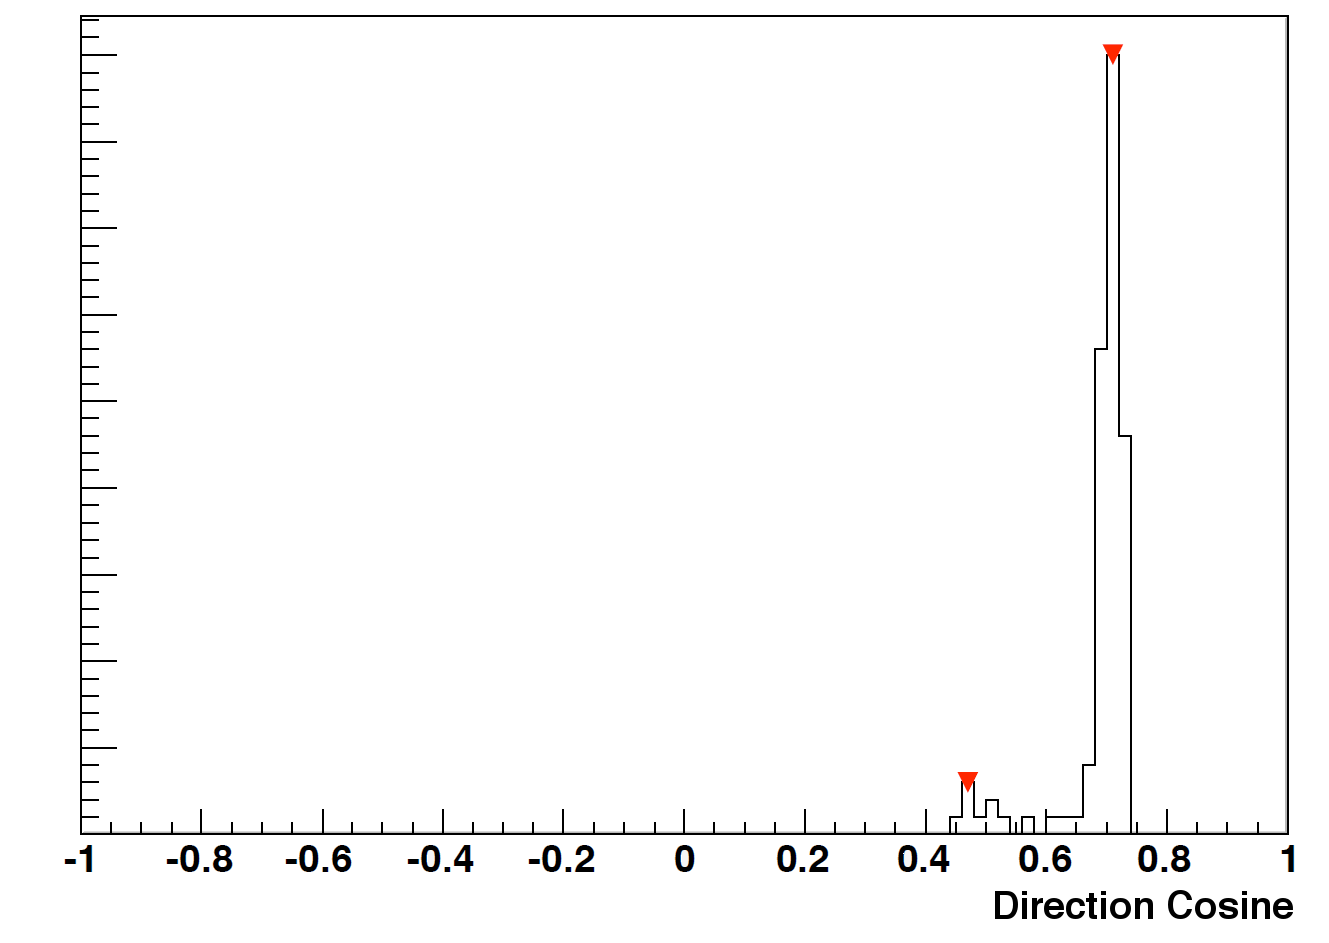
\includegraphics[width=0.7\textwidth]{chapters/otheralg_images/kdtree-peaks}
    \caption{\label{fig:kdtree_peaks}Histogram of direction cosines (the y axis is an arbitrary value corresponding to the number of samples of the direction cosine) as the KDTree algorithm begins to round a corner between two tracks. The right-most peak corresponds to the first line followed, with a large number of samples. When the second peak begins to form, and can be detected by the TSpectrum peak search algorithm, the KDTree reconstruction algorithm is terminated, and a track candidate is reported.}
\end{figure}

When the simple KDTree-based algorithm hits a vertex, it tends to follow the track around the vertex due to the very small scale on which it operates (it sees only immediate neighbours, and so cannot determine that it is following a track around a corner). To overcome this limitation, the direction cosines of the line made by the hits of the track were calculated at each step and added into a ROOT histogram. If the algorithm follows a single straight line, a peak begins to build for the direction cosines corresponding to that line. As soon as the algorithm begins to follow a second straight line (i.e. it has rounded the corner) a second peak will form. Figure \ref{fig:kdtree_peaks} shows a direction cosine histogram in which a second peak is beginning to form, indicating that the algorithm has started to follow a second straight line.

Using this information, the algorithm was terminated when a second peak was seen in the histogram of direction cosines, determined by running a search using the ROOT TSpectrum one-dimensional peak search algorithm. At this point, the last few hits of the track candidate were marked as unallocated, until the direction cosine of the remaining hits in the track candidate had direction cosines corresponding to the first peak. The algorithm was then re-run to attempt to pick up the second track.

While this algorithm was capable of finding straight line structures, the method described above for detecting corners was insufficient to prevent contamination of track candidates with hits from another particle, and the cellular automaton proved to be faster and more efficient, while employing some of the same techniques. The KDTree algorithm was able to reconstruct a limited number of toy tracks from the \emph{TrackGen} simulation, but was never tested against the \emph{Lamu} simulated neutrino events.

\section{The Hough Transform}
The Hough transform is a method for finding straight lines from a set of points $p_i = (x_i, y_i)$ in the $xy$-plane~\citep{Hough1959}. Each point $(x_i, y_i)$ is transformed into a sinusoidal curve $r(\theta)$ as follows:
\begin{equation}
    r(\theta) = x_i \cos \theta + y_i \sin \theta
\end{equation}

A two-dimensional histogram is built up of the values of $r(\theta)$ for each point $p$ in the event, and for $\theta$ sampled over the range $(0,\pi)$. Points lying on the same straight line are described by the same parameters $r,\theta$ and a peak builds up at each such set of parameters that corresponds to a line in the original event. In this way, the process of finding straight line structures in an image (or event) is reduced to the task of finding peaks in a two-dimensional histogram. Figure \ref{fig:hough_histogram} shows one such histogram for a toy event with two tracks. Note that due to the periodic nature of the sine and cosine functions, a peak at a value of $\theta=0$ will be duplicated at $\theta=\pi$; this means that the Hough transform yields lines that extend infinitely in both directions, rather than vectors that would correspond more closely to the accepted idea of a track in particle physics.

\begin{figure}
    \centering
    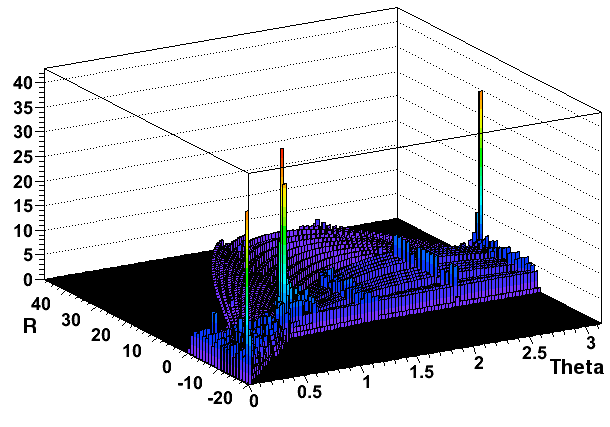
\includegraphics[width=0.8\textwidth]{chapters/otheralg_images/hough-histogram}
    \caption{\label{fig:hough_histogram}Example of a histogram produced when the Hough transform is applied to a toy event containing two straight line tracks. Peaks correspond to the values of $r$ and $\theta$ that parametrise the lines. See the main text for discussion.}
\end{figure}

It should be noted, however, that the Hough transform provides only the parameters of a line; it does not perform clustering, i.e. the allocation of hits to track candidates. This must be done after running the Hough transform by finding any hits that lie close to the line and allocating them to a cluster. Furthermore, the Hough transform yields infinitely long lines; there is no indication of where in an event a track may start or finish. Due to these limitations, the Hough transform was considered to be insufficient for the purposes of track reconstruction in Liquid Argon, where knowledge of the start and end points of tracks is critical to the analysis. In particular, in the absence of a well-defined primary interaction vertex, the Hough transform provides insufficient information to correctly and reliably reconstruct the tracks of a neutrino event.

\section{Graph Clustering Algorithms}
One approach to extracting information from a 3D point cloud that was considered was to build a graph (in the mathematical sense of a connected network of nodes with possibly weighted edges) where each node was a point in the data set, and each edge was weighted by the distance between the nodes it connects.

Given such a graph, it is possible to analyse the data in a number of ways, including determining the shortest path between two nodes using standard shortest path algorithms, for example Dijkstra's algorithm~\citep{Dijkstra1959}. Using the networkx\footnote{\url{http://networkx.github.io/}} Python library for graph manipulation, this could be trivially applied to data from the \emph{TrackGen} or \emph{Latte} simulations.

Given two extreme points in the event (e.g. a point close to the origin, and a point near the edge of the event) the shortest path algorithm provides a preliminary clustering of a track, containing those hits that lie on the shortest path between the ends of the track, however it is strongly dependent on a good seed point. Use of this approach in conjunction with the feature detection algorithms outlined in chapter \ref{sec:latte_feature_detection} may give reasonable seed points for this technique. There still remains the issue of assigning hits surrounding the core to the track that was found, and the cellular automaton once again outperforms in this area.

No substantial analysis of this approach was performed, in part because the cellular automaton provided a promising approach to track reconstruction, and because there are many possible algorithms that could be run against a network or graph of spatial data, and it was not clear which possibilities would give the best results. The use of this technique to cluster or classify showers in a liquid Argon volume was briefly considered, but again no significant characterisation of the properties or mechanics of such an algorithm was performed.

